\documentclass{tum_report}
% -----------------------------------------------------------------------
%  Extra packages that may not be in the template already
% -----------------------------------------------------------------------
\usepackage{amsmath}
\usepackage{amssymb}
\usepackage{float}
\usepackage{graphicx}
\usepackage{enumitem}
\usepackage{verbatim}
\usepackage{booktabs}
\usepackage{array}
\usepackage{xcolor}
\usepackage{hyperref}

\begin{document}

    \ministry{MINISTRY OF EDUCATION, CULTURE AND RESEARCH\\OF THE REPUBLIC OF MOLDOVA}


\university{\textbf{Technical University of Moldova}}
\faculty{\textbf{Faculty of Computers, Informatics and Microelectronics}}
\department{\textbf{Department of Software Engineering and Automatics}}

\title{Computer Graphics}

\year{2026}

\begin{titlepage}
    \centering

    % --- Logo ---
    
\includegraphics[width=0.25\textwidth]{./UTM_Logo.png}\par\vspace{1cm}

    % --- Ministry and University info ---
    {\bfseries
        \textsc{\ministryname} \\[0.15cm]
        \universityname\\[-0.01cm]
        \facultyname\\[-0.01cm]
        \departmentname
    }\par


    \vspace{2.5cm}

    % --- Student info ---
    \textbf{Mihail Pancenco} \textbf{FAF-243}\par

    \vspace{-0.5cm}

    % --- Title section ---
    {\Large \textbf{Report}\par} \normalsize	
    \vspace{0.5cm}
    {\normalfont\Large \textit{Laboratory work n. 1}\par}
    \vspace{-0.5cm}
    \Large \textit{of Operating Systems}\par \normalsize	

    \huge \textit{The OS as a Resource Manager}\par \normalsize	
    

    \vspace{3cm}

    % --- Checked by section ---
    \begin{flushright}
        {\normalfont
            Supervisers:\par
            \textbf{Dumitrașcu Marius}, \textit{University assistant}\par
            \textbf{Reițman Patricia}, \textit{University assistant}\par
            DISA, FCIM, UTM
        }
    \end{flushright}
    
    

    \vfill{}

    % --- Footer ---
    \textbf{Chișinău -- \degreeyear}\par

\end{titlepage}


    \clearpage

    \addtocontents{toc}{\protect \thispagestyle{empty}}
    \tableofcontents
    \thispagestyle{empty}
    \clearpage

% =======================================================================
\chapter{Introduction}
% =======================================================================


% In today’s lecture you met the operating system as the manager that stands between your programs and the hardware.
% In this lab you will see that manager at work with your own eyes, on the provided Linux virtual machine.
% You will watch the four core jobs of any OS (managing files, processes, memory and devices) happen live in the terminal,
% and you will write down what you observe (not just which command you typed).
\par In this laboratory work, we will explore the operating system as a manager that stands between programs and hardware.
We will see the four core jobs of any OS (managing files, processes, memory and devices) happen live in the terminal, and we will document our observations.

\chapter{Before we start}

\par Before we start, we need to log in the Ubuntu in the Virtual Machine. Then, create a working folder and keep a file called report.md opened beside the terminal.

\begin{figure}[H]
    \centering
    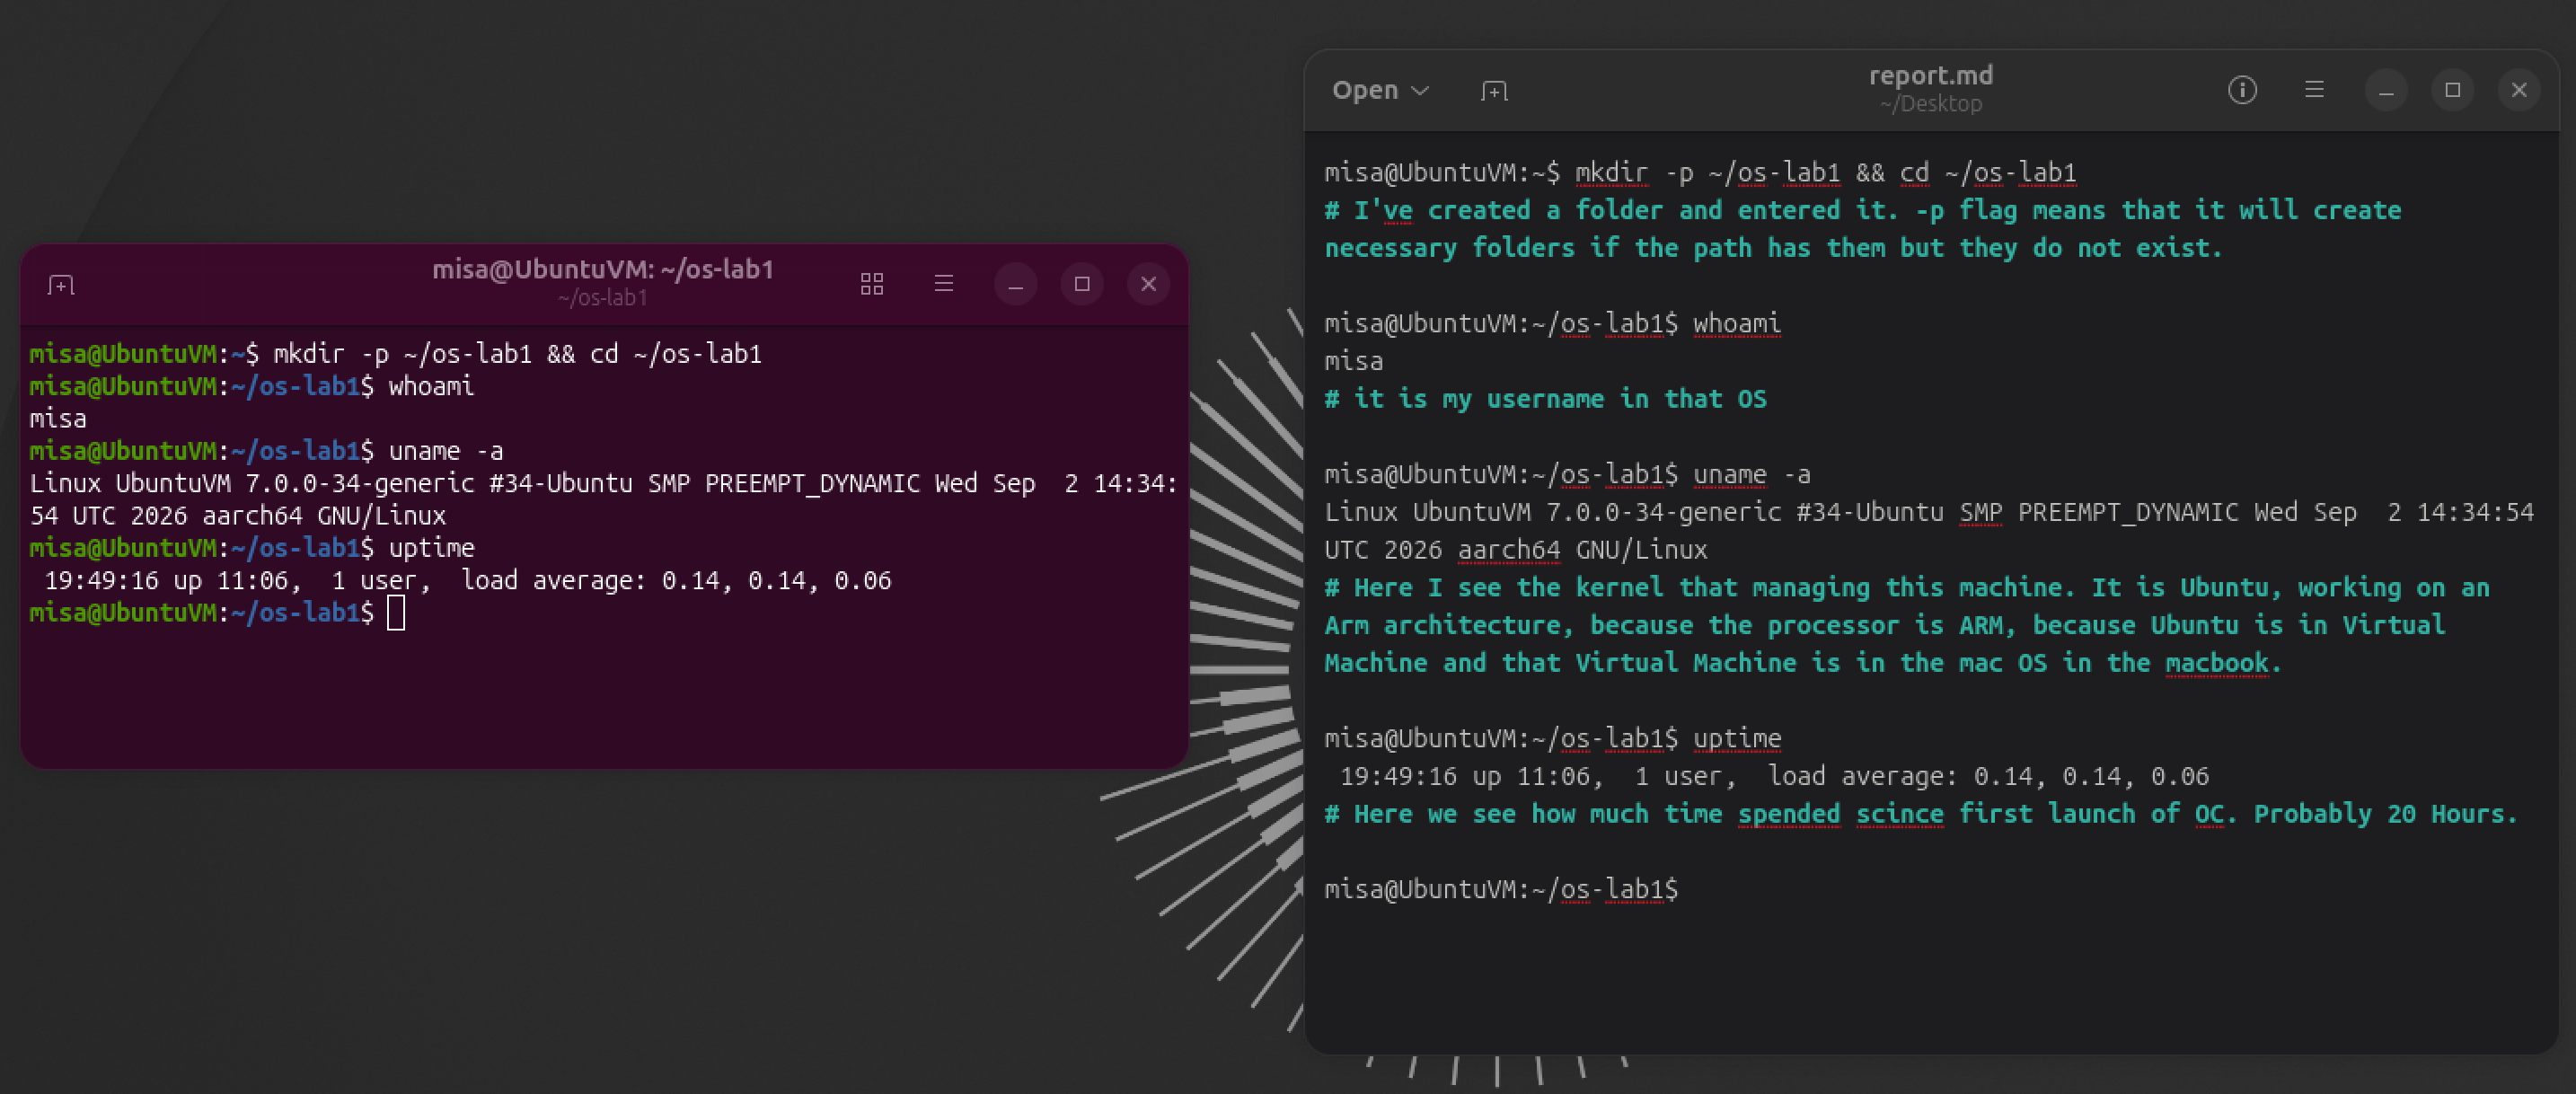
\includegraphics[width=0.82\textwidth]{./img/img_01.png}
    \caption{Basic configuration of OS and observations in report.md}
    \label{fig:label_01}
\end{figure}

\par So, my username is 'misa', I use Ubuntu in Virtual MAchine which is running on macbook real machine. Ubuntu is running already almost 20 hours. 

\chapter{Exploting the OS}
\section{Files and directories}


\par The OS turns a raw disk into a tidy tree of named files with owners and permissions. We will explore that tree and change it.

\par To see where we are now, we use \texttt{pwd} command. The \texttt{ls -la} will show the root of the whole tree. \texttt{-l} flag means to show in a list, the \texttt{-a} flag meand to show all, even hidden file and folders.

\texttt{ls -la \textasciitilde} will show the tree of the home directory as \texttt{\textasciitilde} is the alias for that directory. The \texttt{cd /etc} will enter into the etc folter and \texttt{ls | head} will show first 10 results of ls, as the result of \texttt{ls} command goes to \texttt{head} command and this command shows only top 10 results.

\begin{figure}[H]
    \centering
    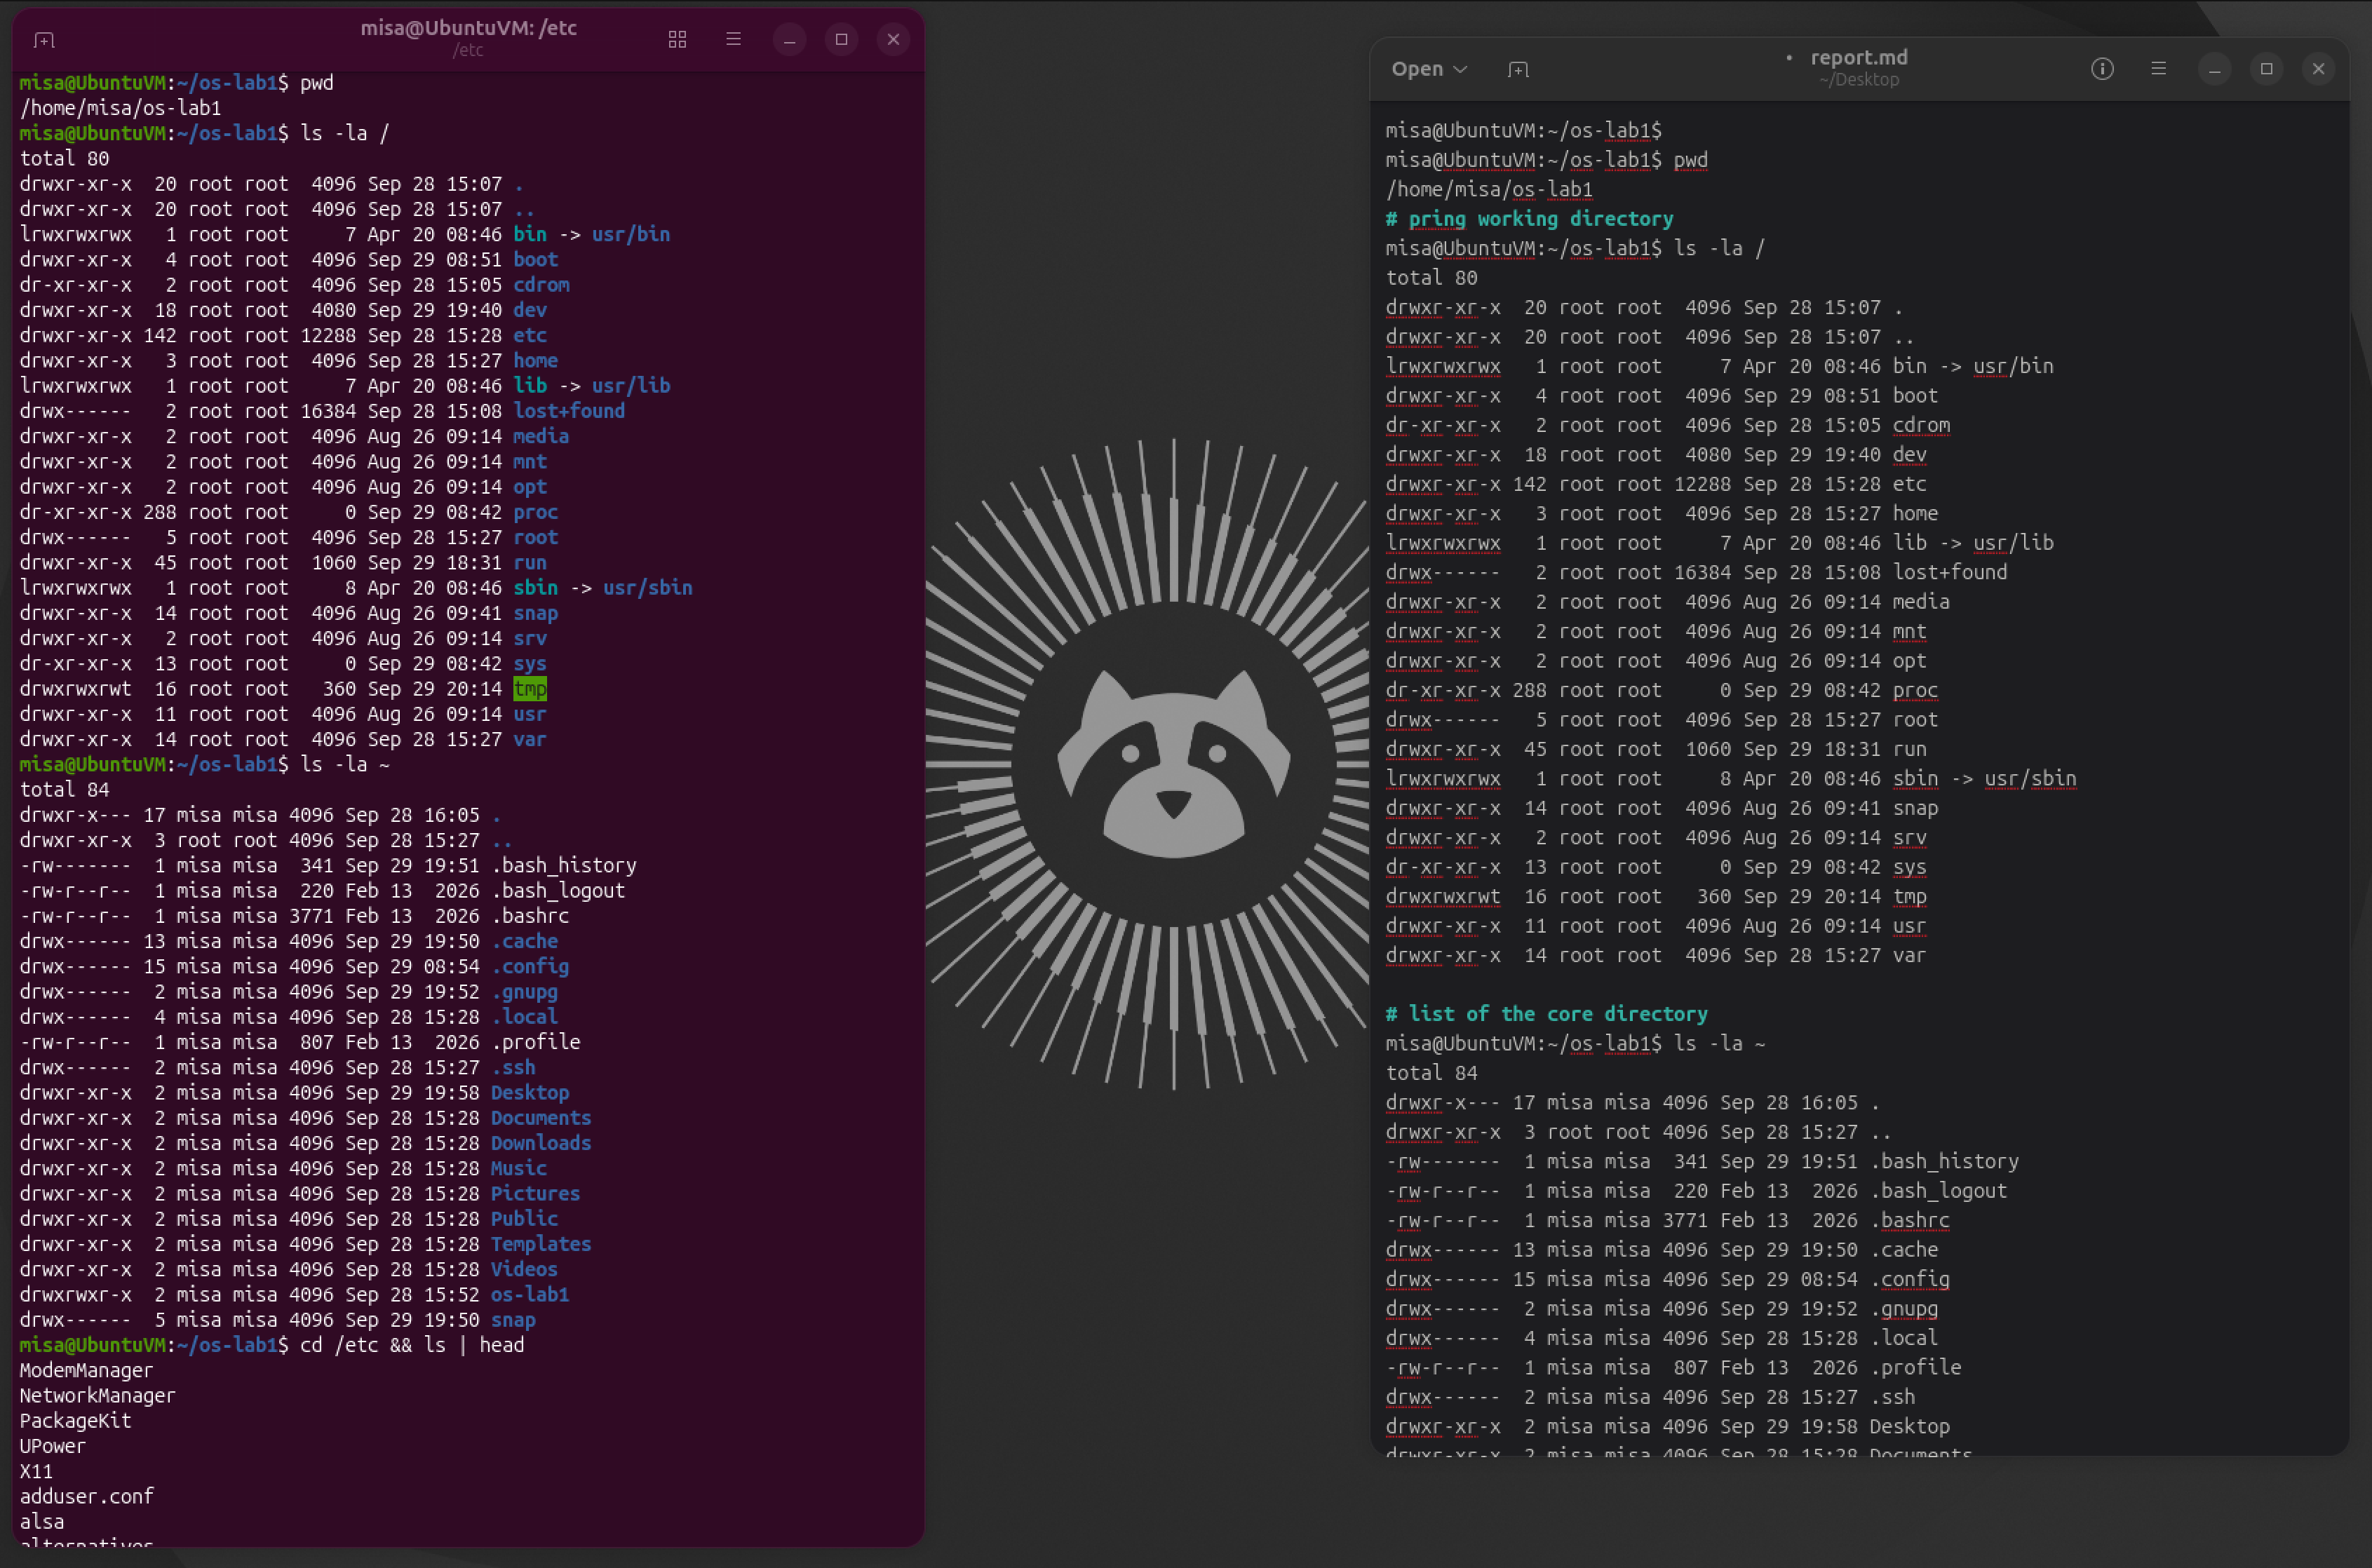
\includegraphics[width=0.82\textwidth]{./img/img_02.png}
    \caption{Exploring the file tree}
    \label{fig:label_02}
\end{figure}

\par Moving forward, now we will not just explore, but create, copy, rename and remove something and see the tree changes.
\texttt{cd ~os-lab1} will enter the \texttt{os-lab1} folder. Then we will create a \texttt{demo} folder. There create a file named \texttt{note.txt} containing the text \texttt{"hello operating systems"}. Then we will create a copy of that file, rename the copy, see the list of tree in that directory and finally remove the copied renamed file.


\begin{figure}[H]
    \centering
    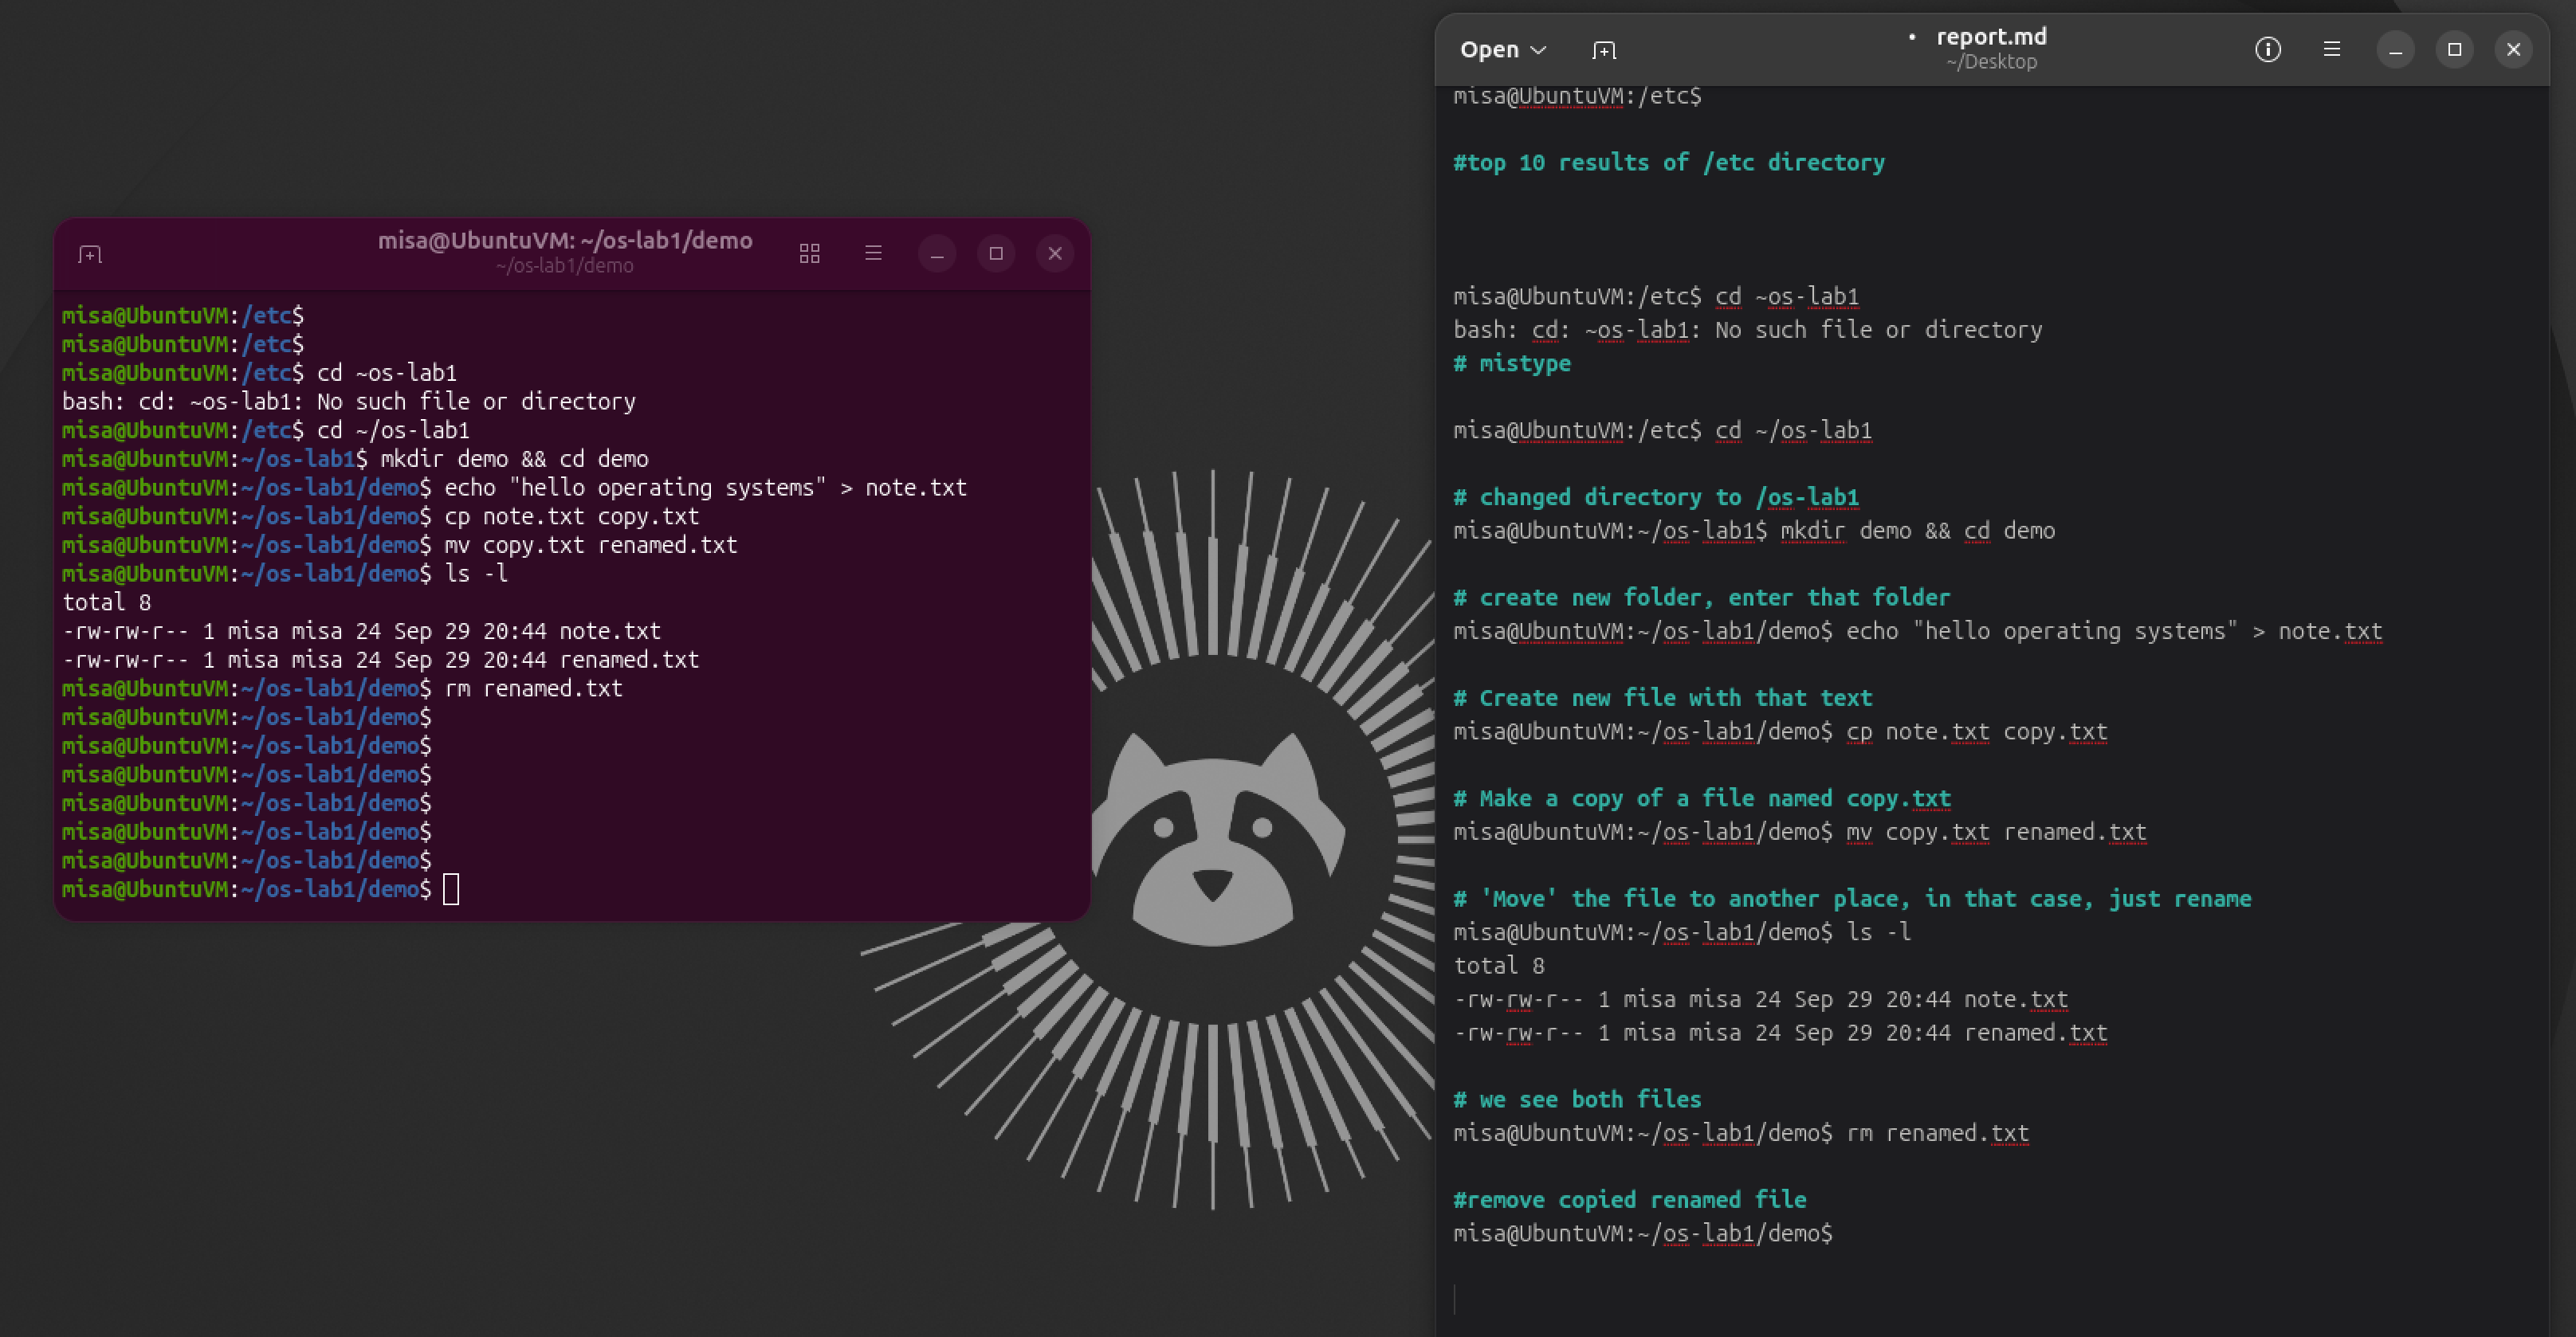
\includegraphics[width=0.82\textwidth]{./img/img_03.png}
    \caption{Using the file tree}
    \label{fig:label_03}
\end{figure}

\par Now we explore the ownership permissions. The OS decides who may touch what. We will \texttt{change mod} of file and see what happens in the ouptut of \texttt{ls -l} command. 


\begin{figure}[H]
    \centering
    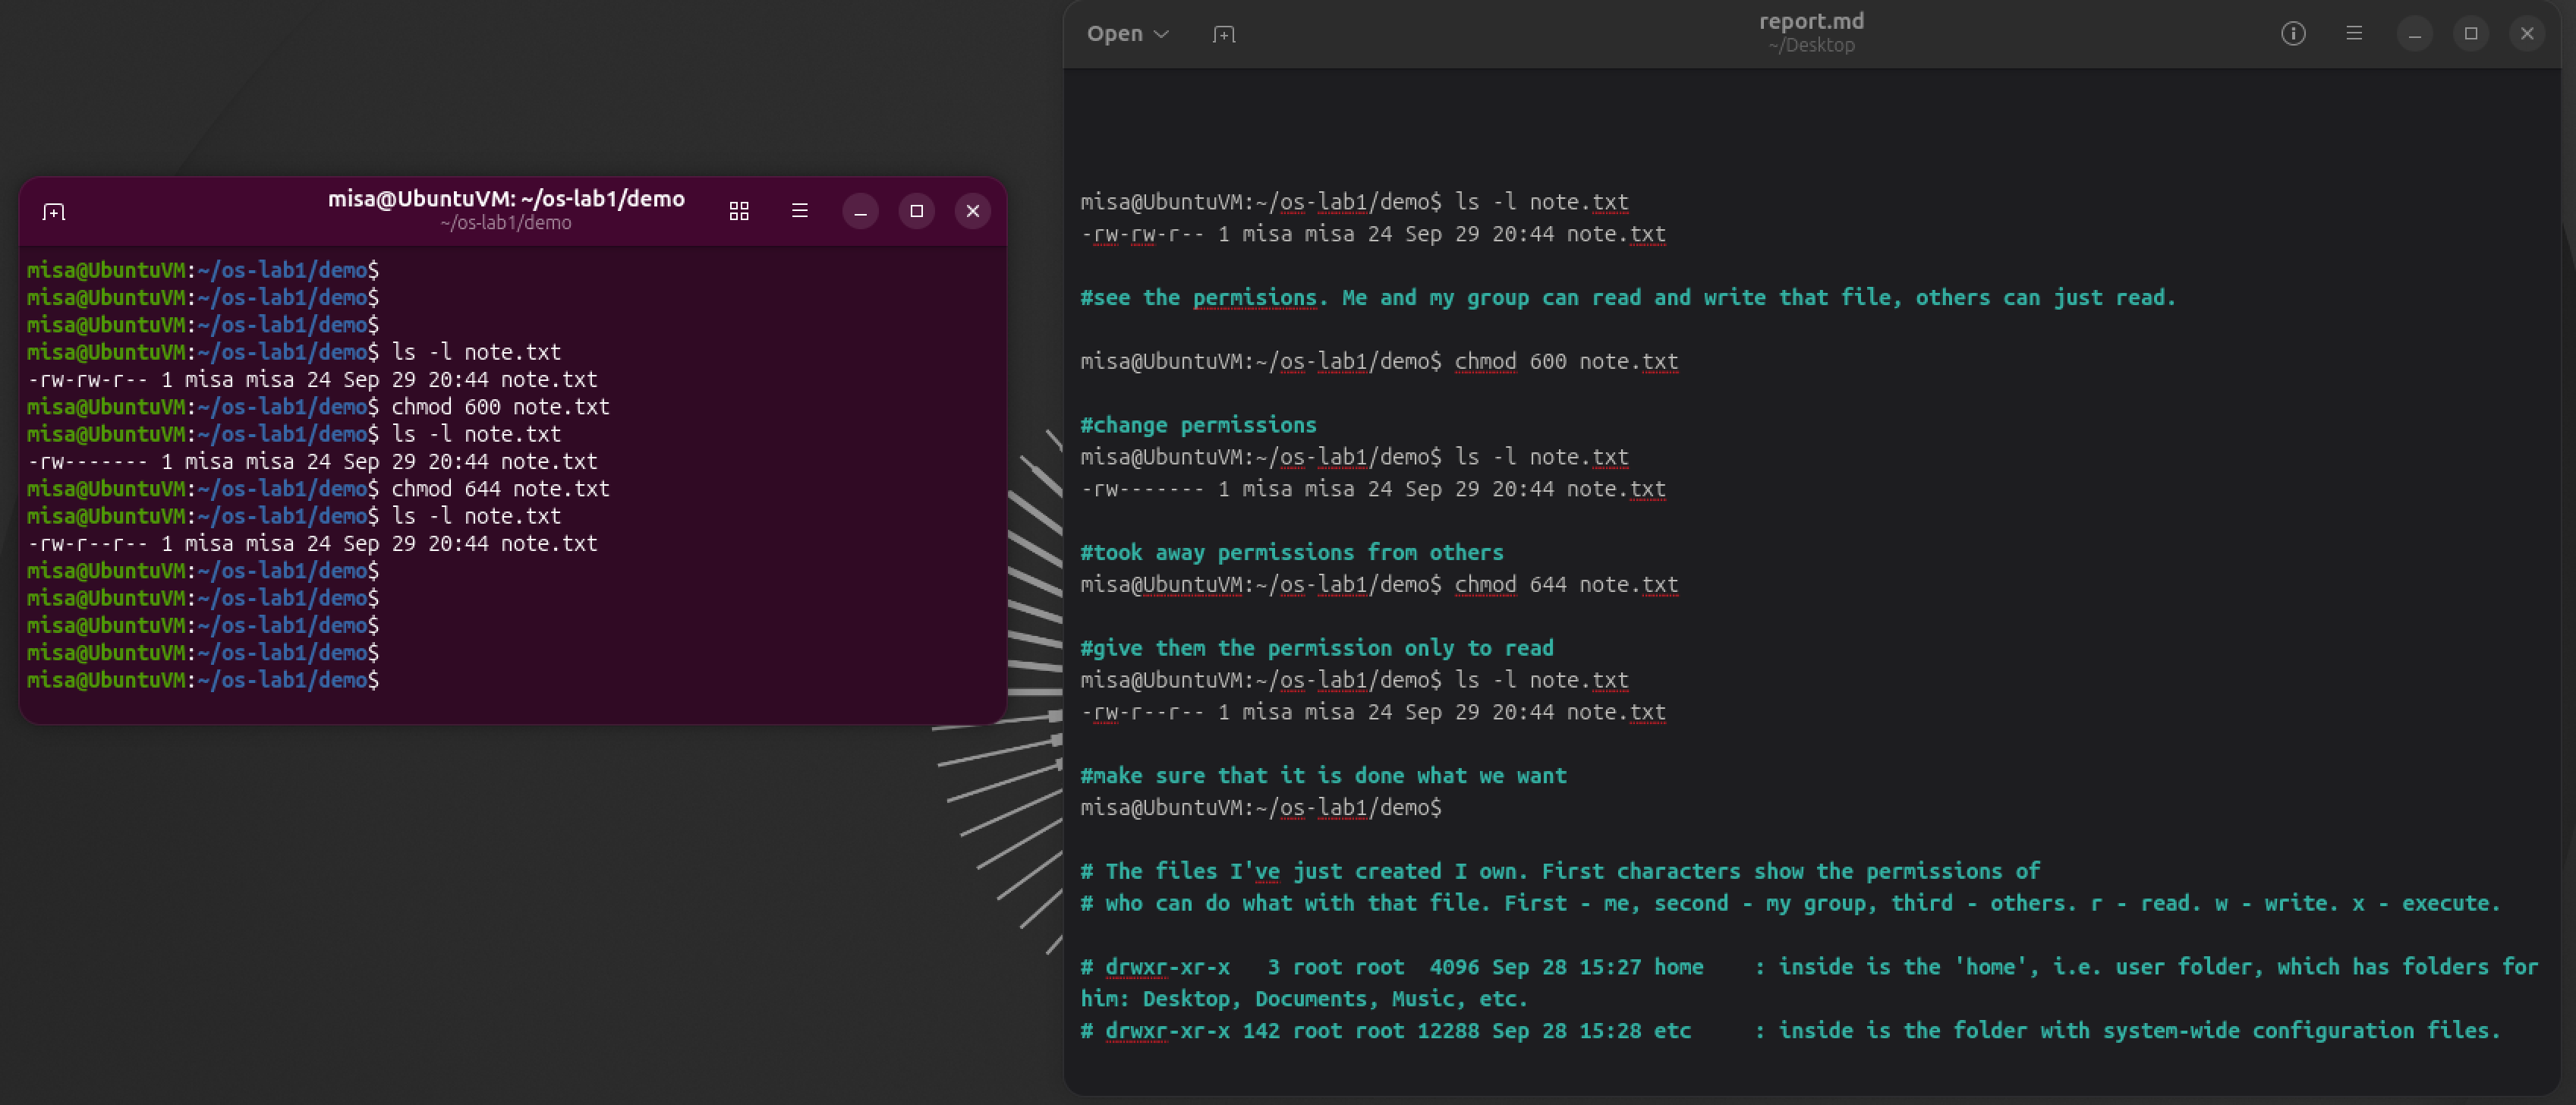
\includegraphics[width=0.82\textwidth]{./img/img_04.png}
    \caption{Edit and explore permissions}
    \label{fig:label_04}
\end{figure}


\section{Processes}
\par Every running program is a process that OS created, isolated and schedules. We will find them, start one and stop it.
\par Firstly, we will see the processes that OS is currently juggling. 


\begin{figure}[H]
    \centering
    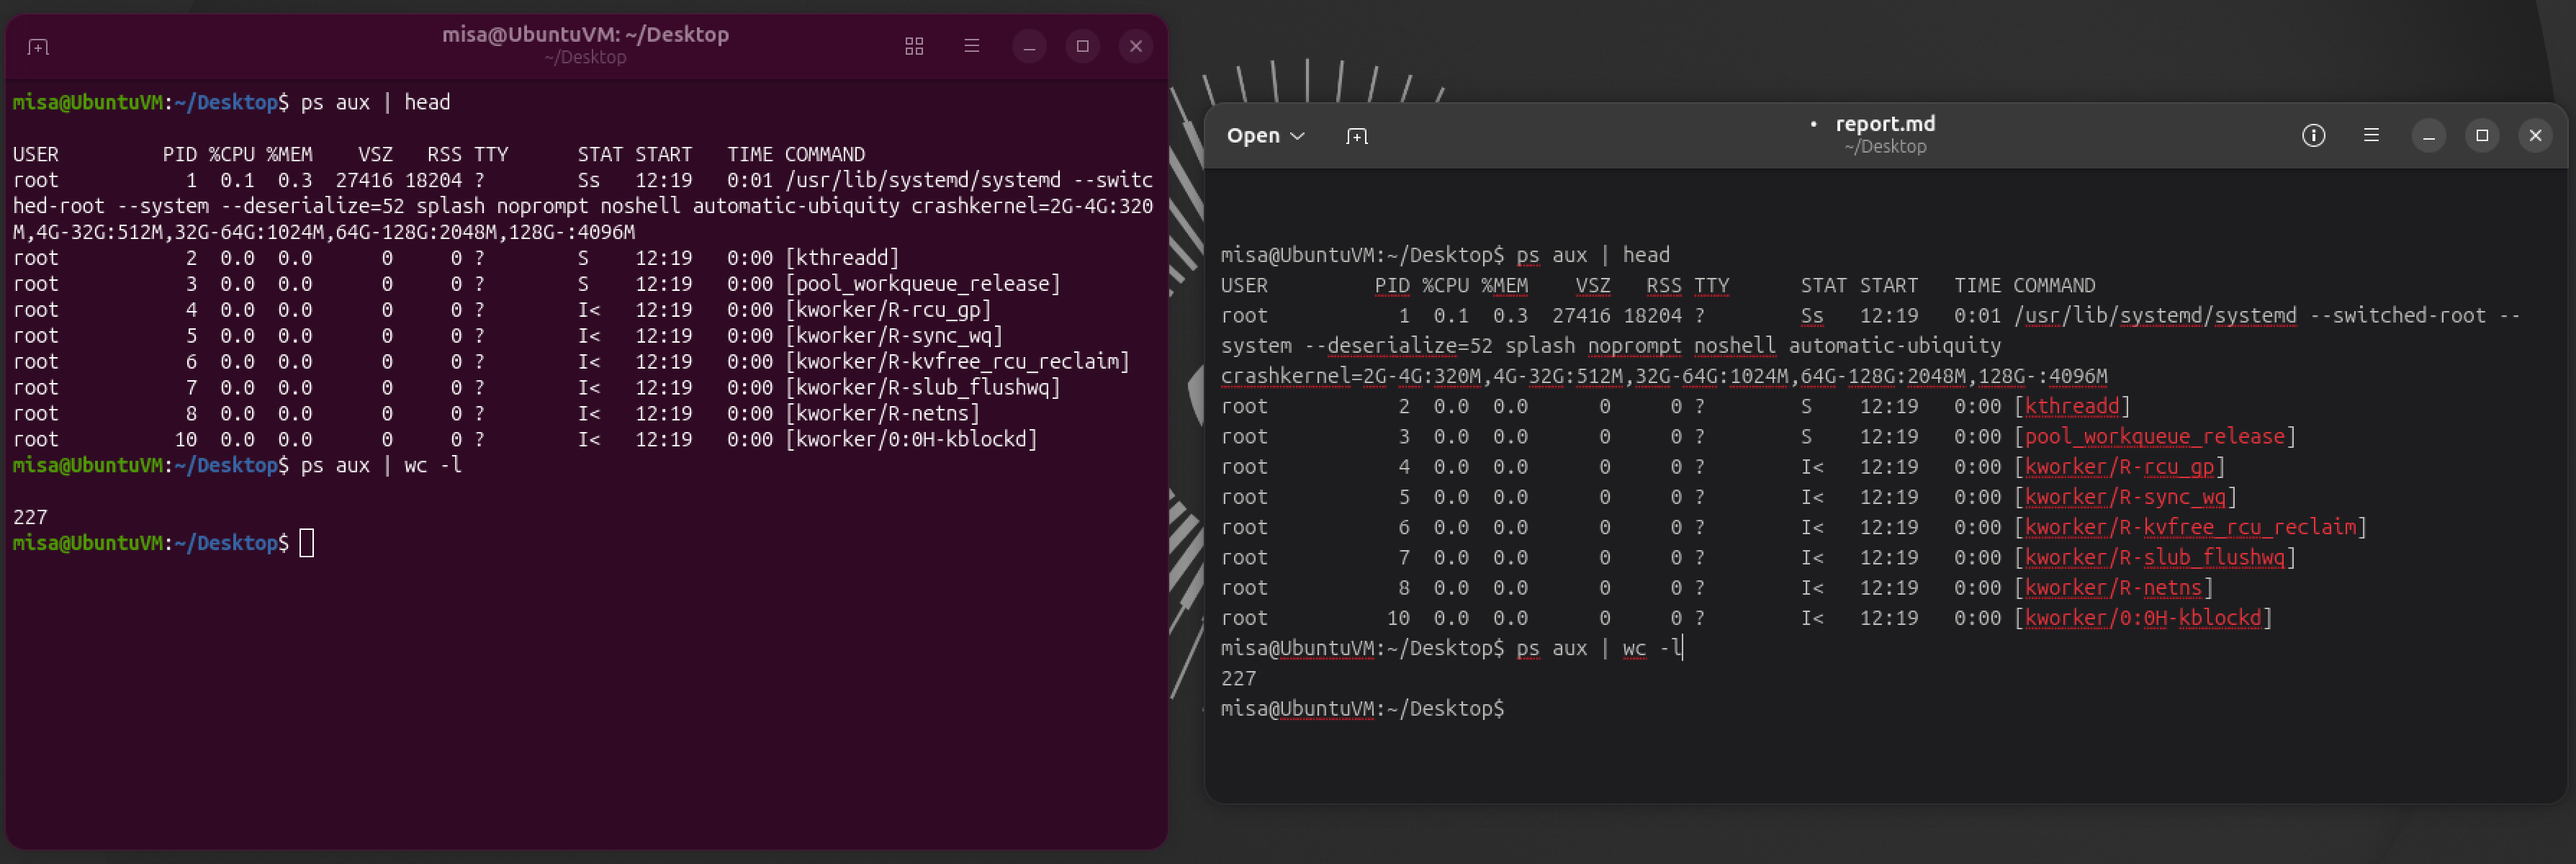
\includegraphics[width=0.82\textwidth]{./img/img_05.png}
    \caption{List the processes the OS is currently juggling}
    \label{fig:label_05}
\end{figure}

\par The OS is currently juggling 227 processes.


\begin{figure}[H]
    \centering
    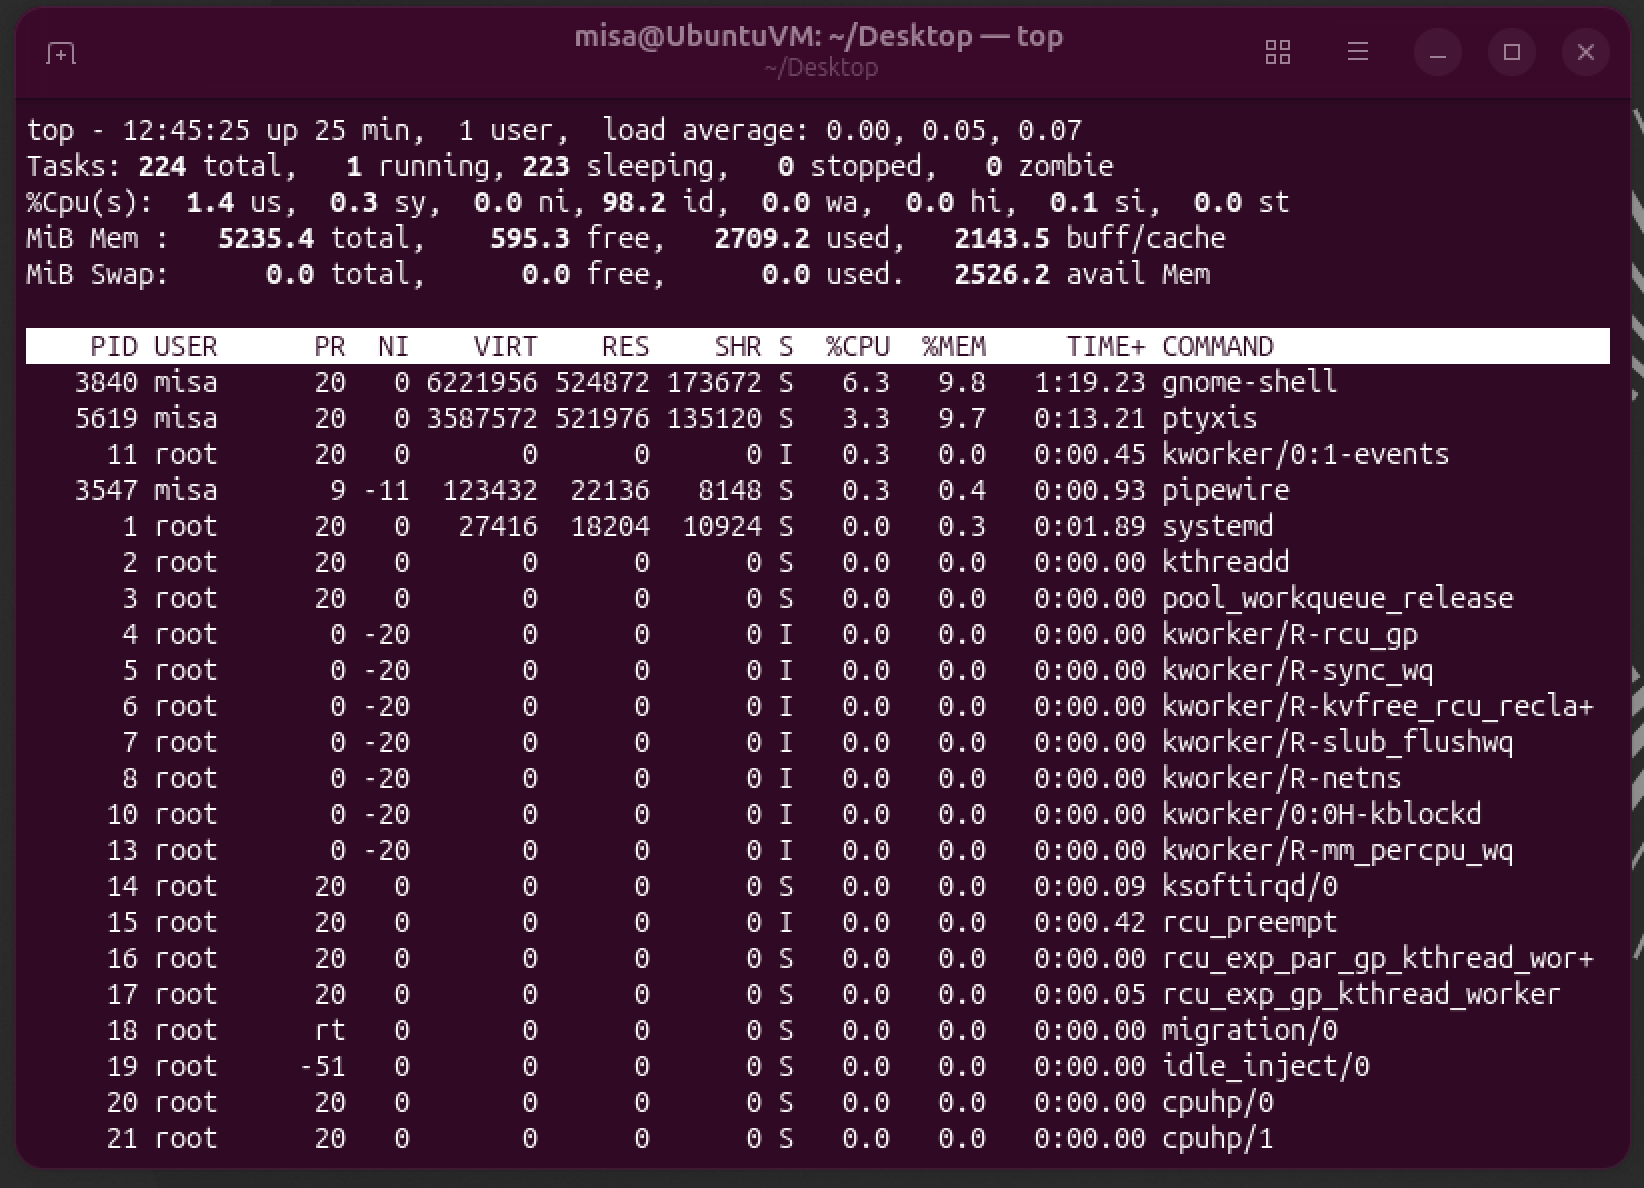
\includegraphics[width=0.82\textwidth]{./img/img_06.png}
    \caption{Output of \texttt{top} command}
    \label{fig:label_06}
\end{figure}

\par Now start the background process, find it and stop it. 


\begin{figure}[H]
    \centering
    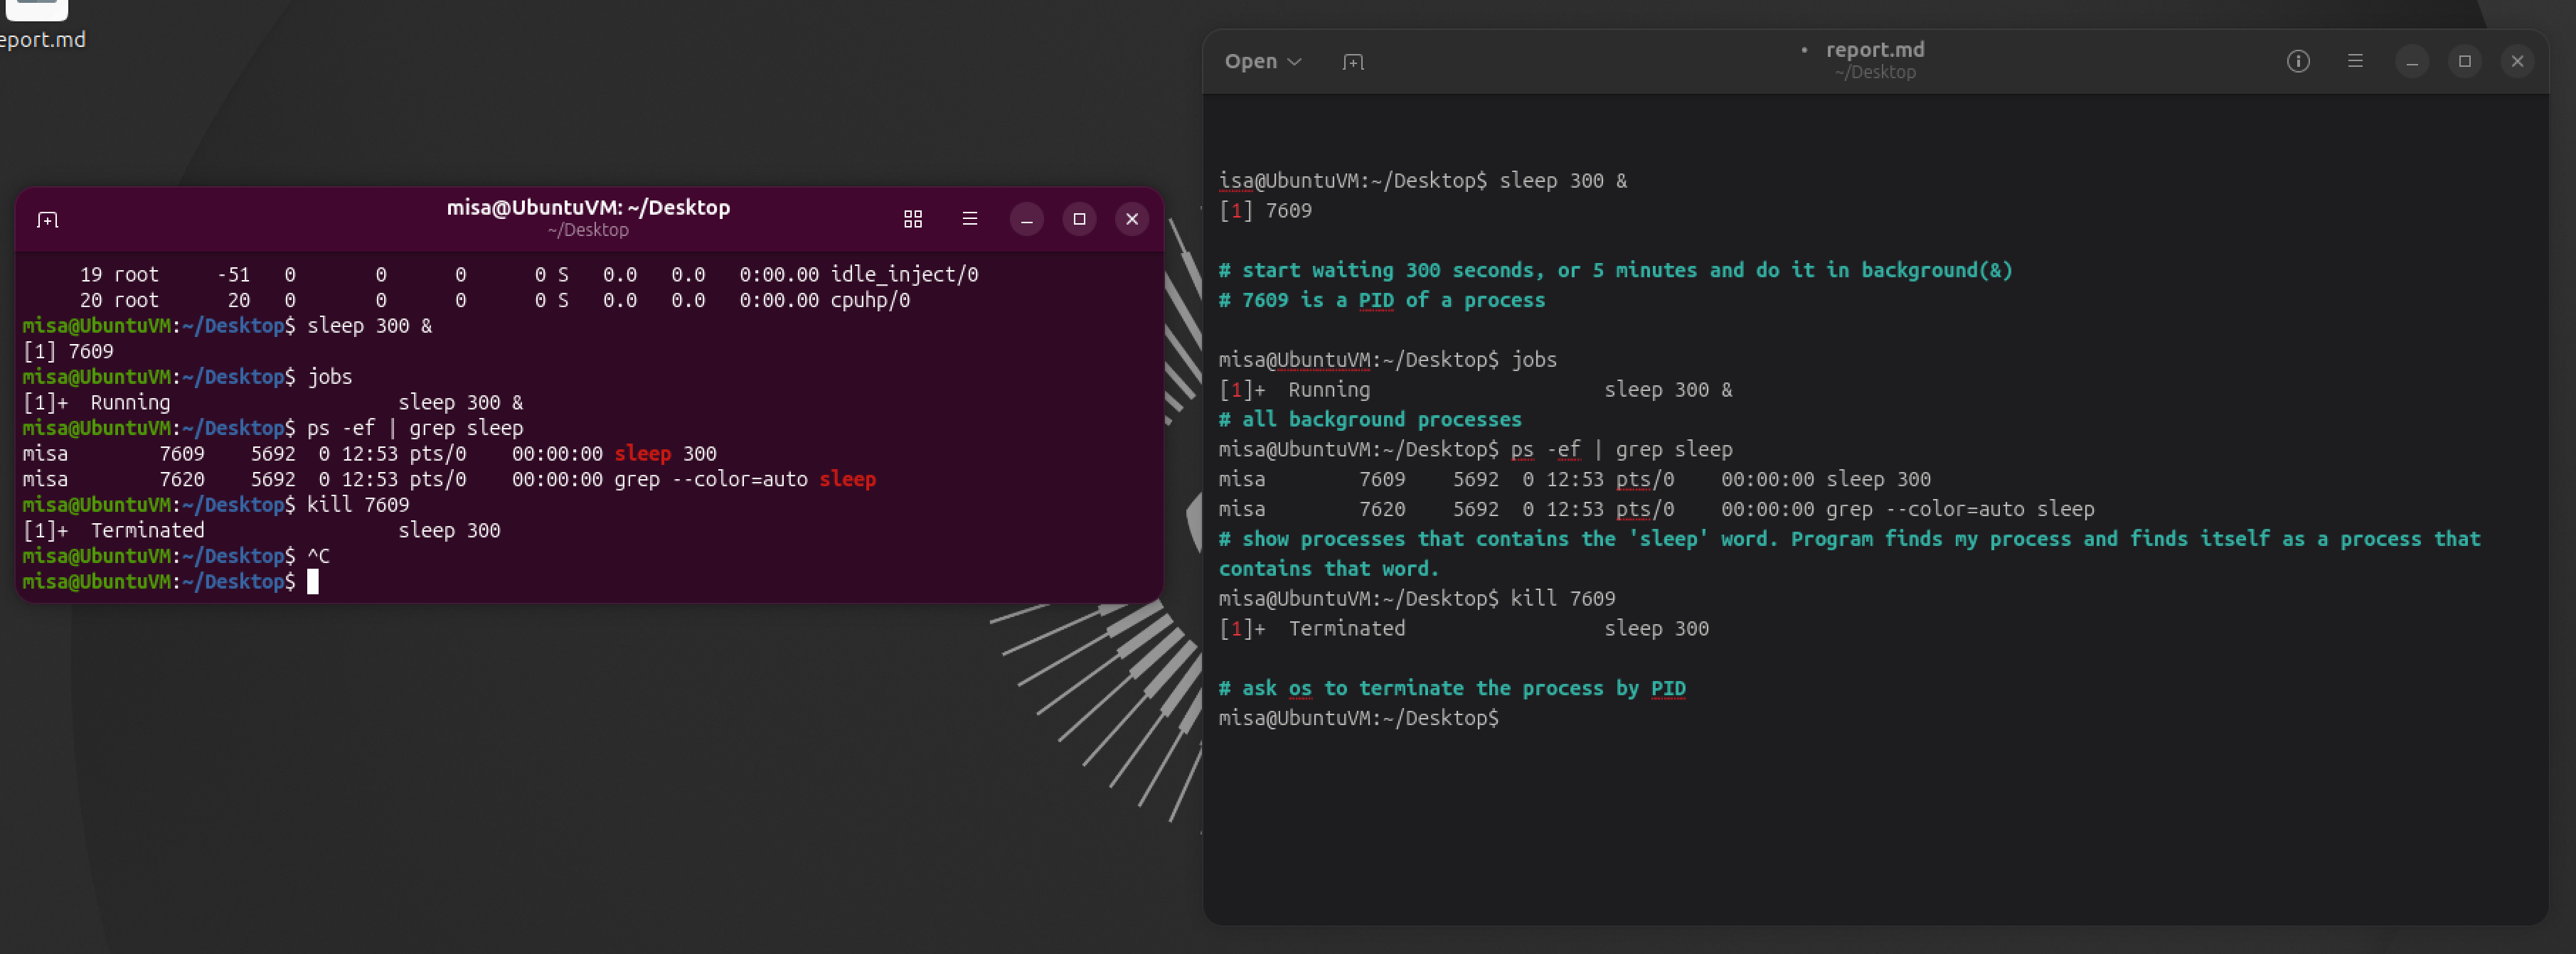
\includegraphics[width=0.82\textwidth]{./img/img_07.png}
    \caption{Start background process, find it and stop it}
    \label{fig:label_07}
\end{figure}

\par The \texttt{ps -ef} shows all processes in a full format, the \texttt{grep sleep} leaves only processes with the name \texttt{sleep}.
\par Now peek at what the kernel exposes about a process through the \texttt{/proc pseudo-filesystem}.


\begin{figure}[H]
    \centering
    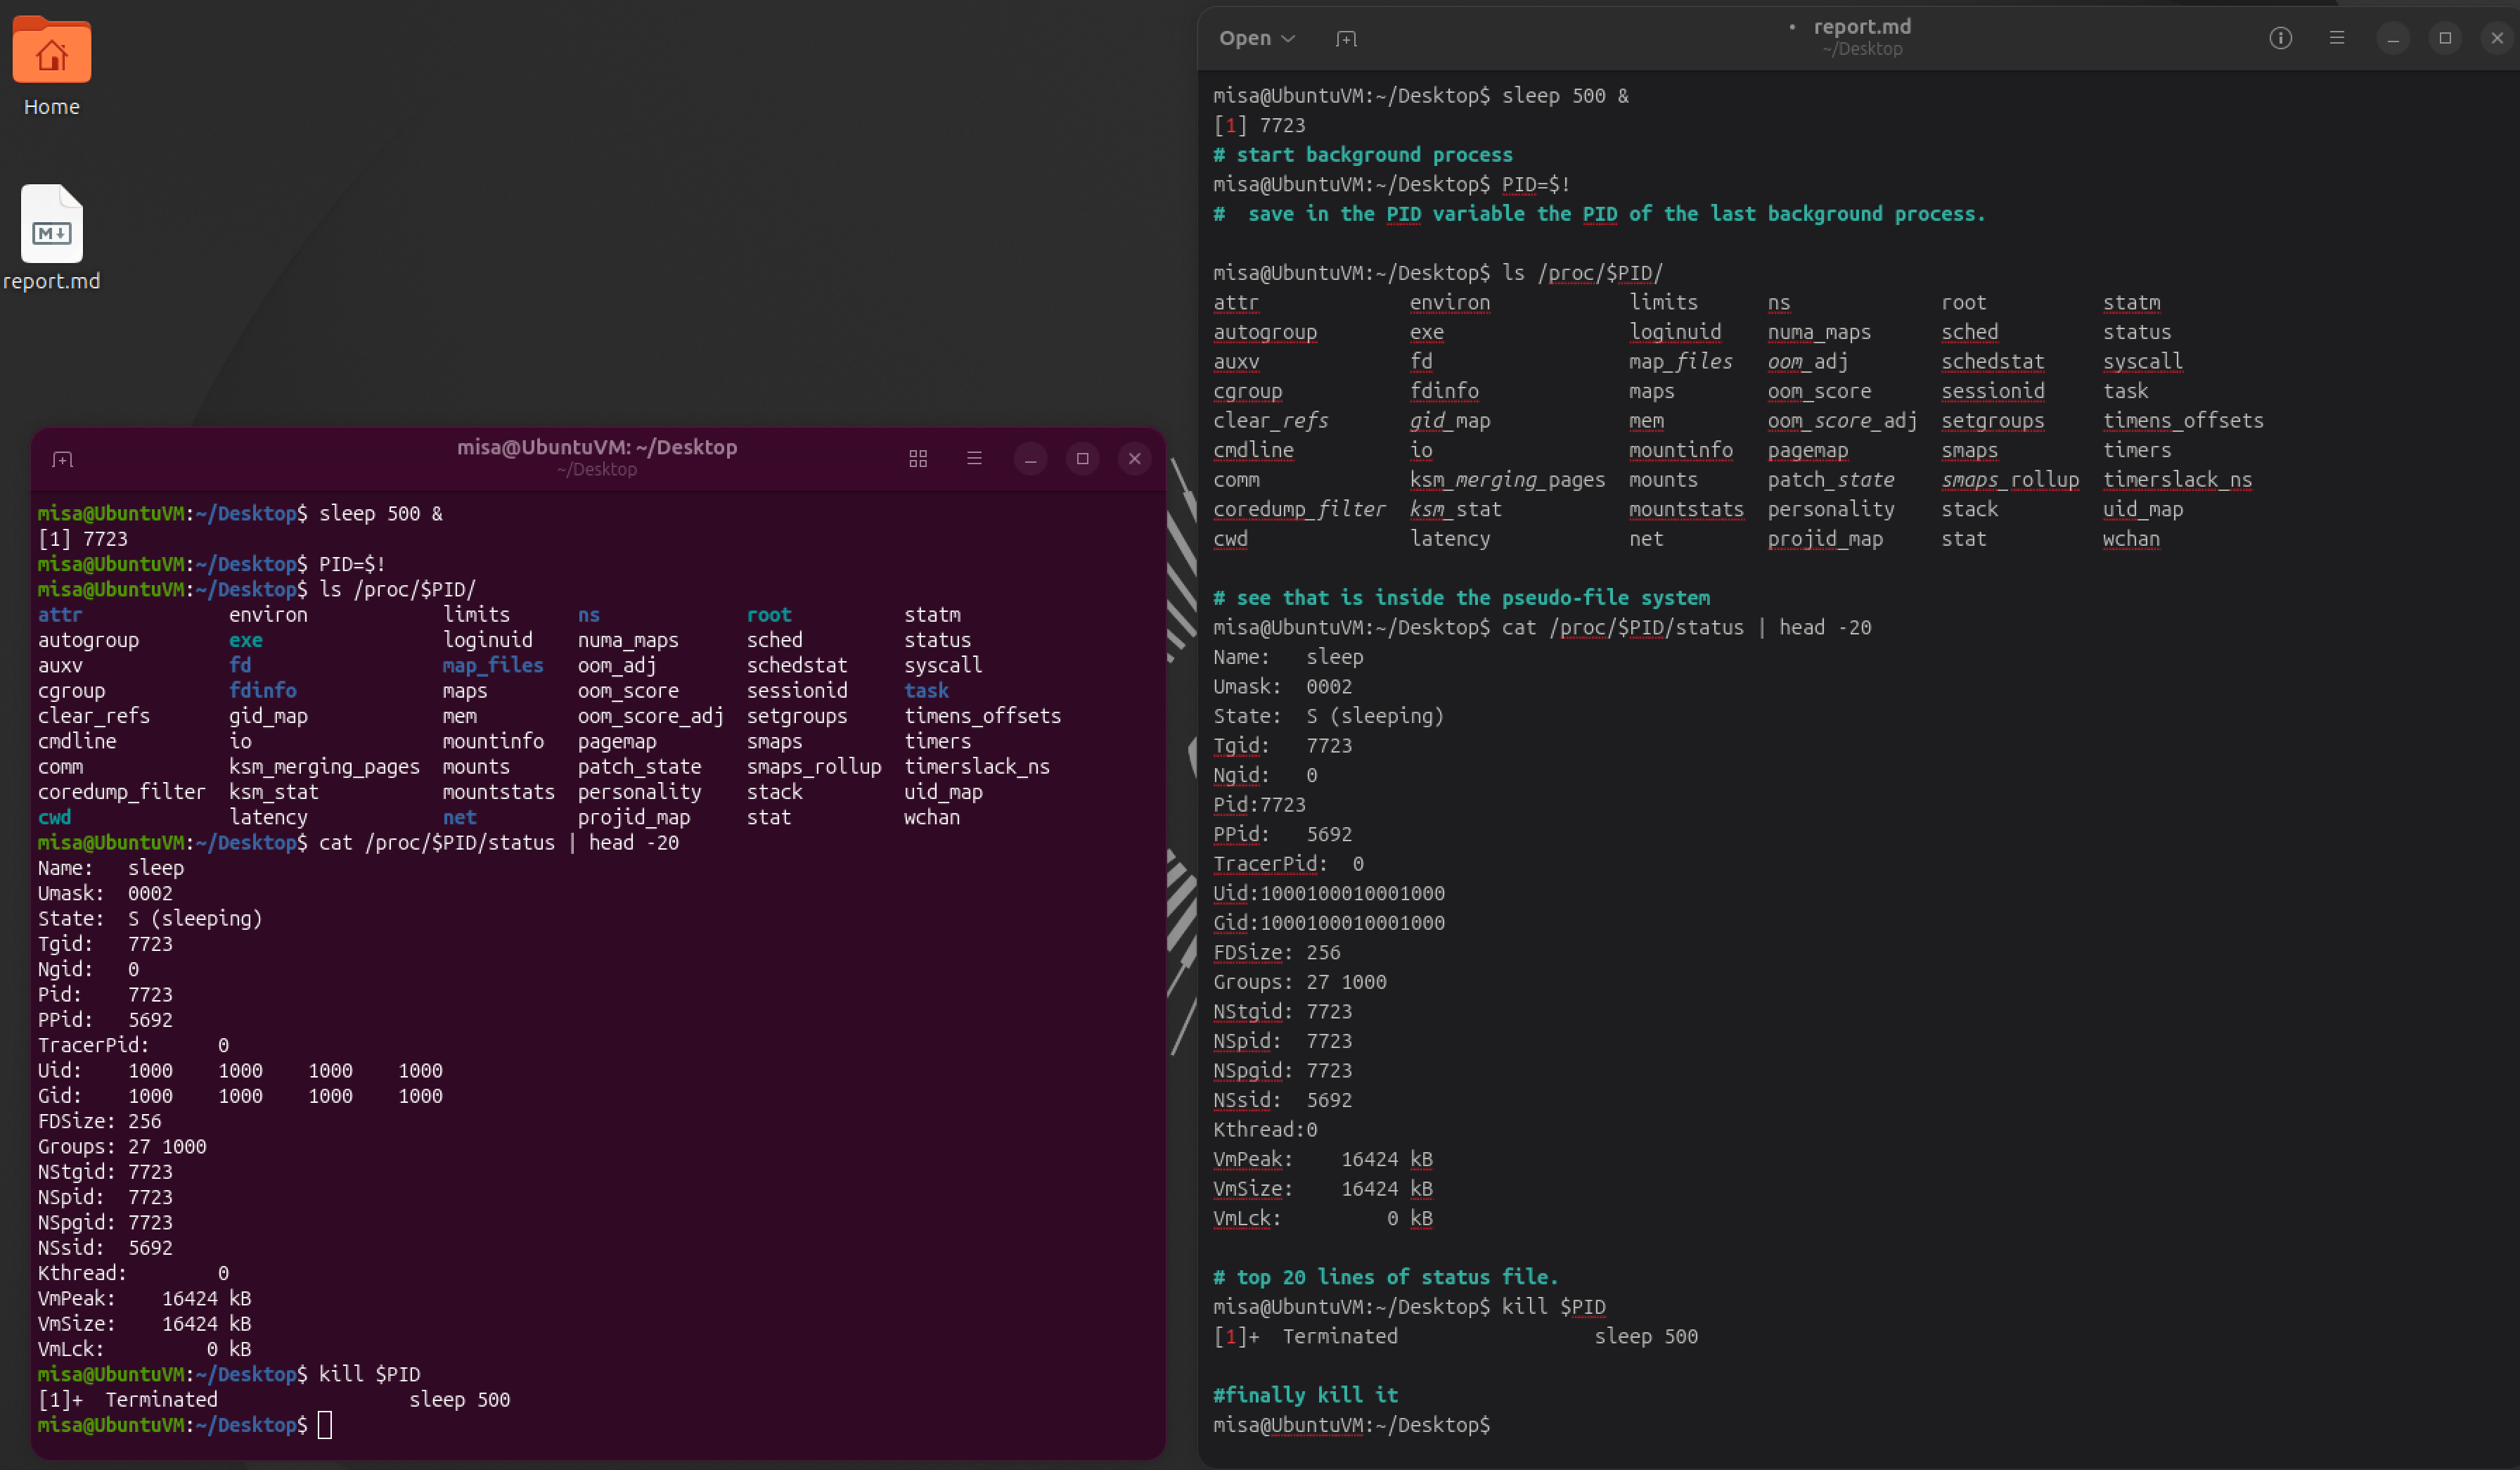
\includegraphics[width=0.82\textwidth]{./img/img_08.png}
    \caption{peek at what the kernel exposes about a process through the \texttt{/proc pseudo-filesystem}}
    \label{fig:label_08}
\end{figure}

\par \texttt{/proc} is a pseudo-filesystem that provides information about running processes and the current state of the Linux kernel through a file-like interface.


\par We notice that the process with PID 1 is \texttt{systemd}, the first userspace process started by the Linux kernel that manages system services. The idle VM had roughly 220--230 running processes. We also notice that the \texttt{sleep} process had the state \texttt{S (sleeping)}, meaning that it was waiting and not actively using the CPU.


\section{Memory}
The OS hands each process its own view of memory and shares the physical RAM between them.


\begin{figure}[H]
    \centering
    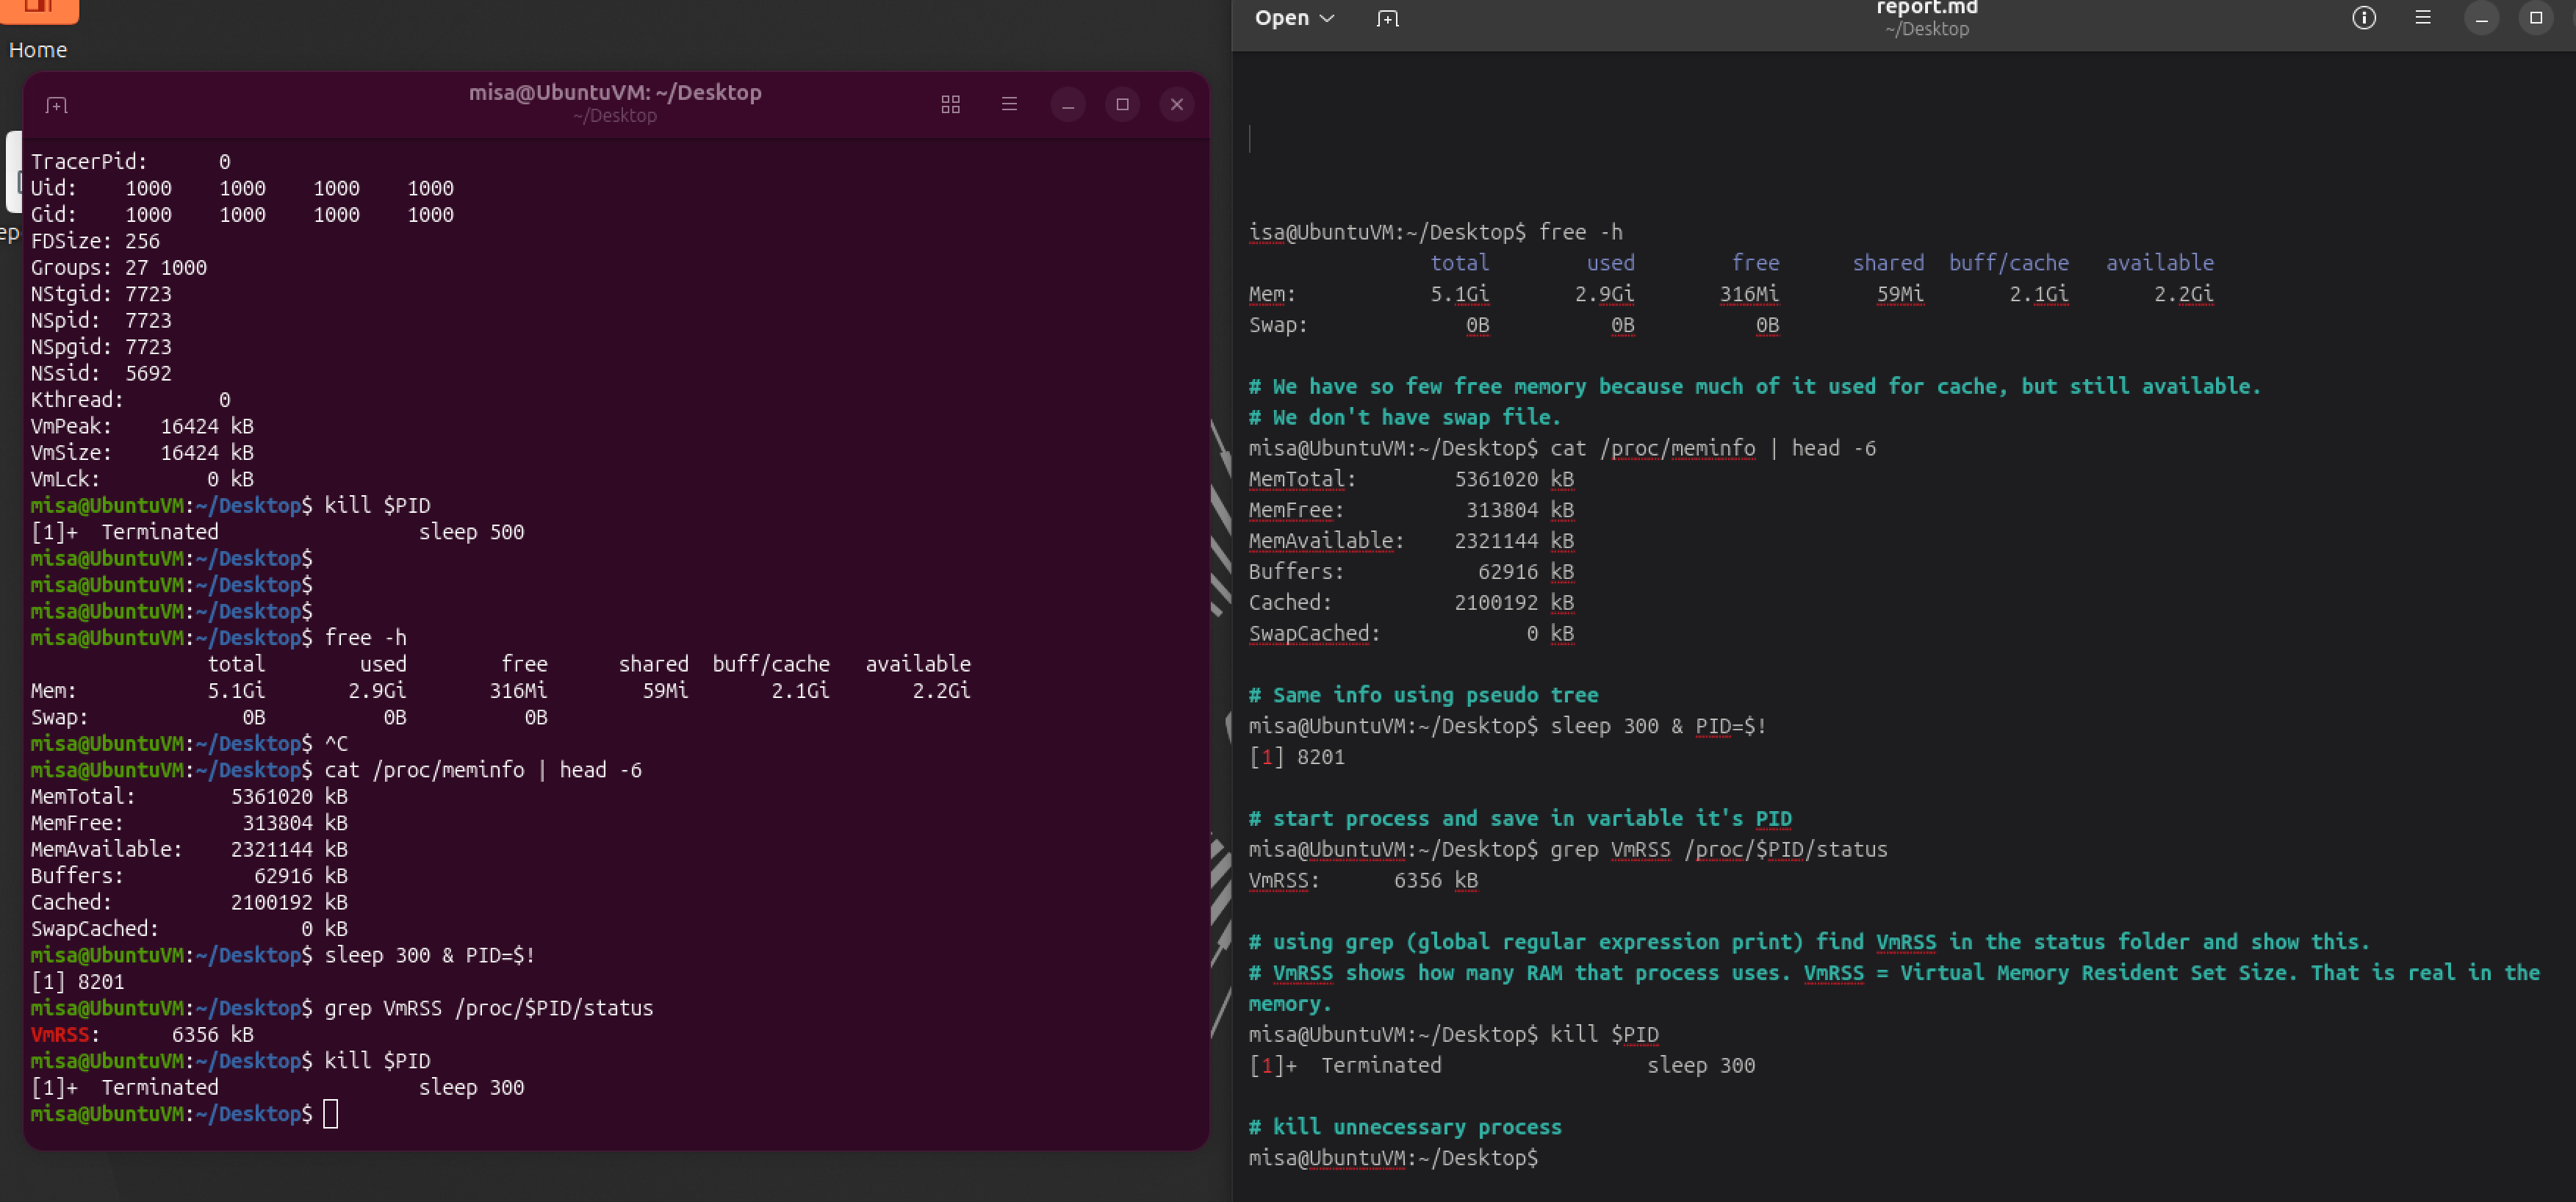
\includegraphics[width=0.82\textwidth]{./img/img_09.png}
    \caption{Memory management}
    \label{fig:label_09}
\end{figure}

\par We notice that the VM has 5.1 GiB of total RAM, with only about 316 MiB completely free. However, about 2.2 GiB is still available because a significant part of the memory is used for cache and can be reclaimed when needed. We also notice that no swap is configured, meaning that no disk space is currently used as an extension of RAM. Using the \texttt{/proc} pseudo-filesystem, we find that a simple \texttt{sleep} process has a VmRSS (Virtual Memory Resident Set Size) of 6356 kB, or about 6.2 MiB of physical RAM. This is surprisingly large considering that the \texttt{sleep} process does almost no actual work.


\section{Devices and storage}

\par The OS hides every disk, terminal and device behind uniform file-like interfaces. That is the "everything is a file" idea of UNIX.


\begin{figure}[H]
    \centering
    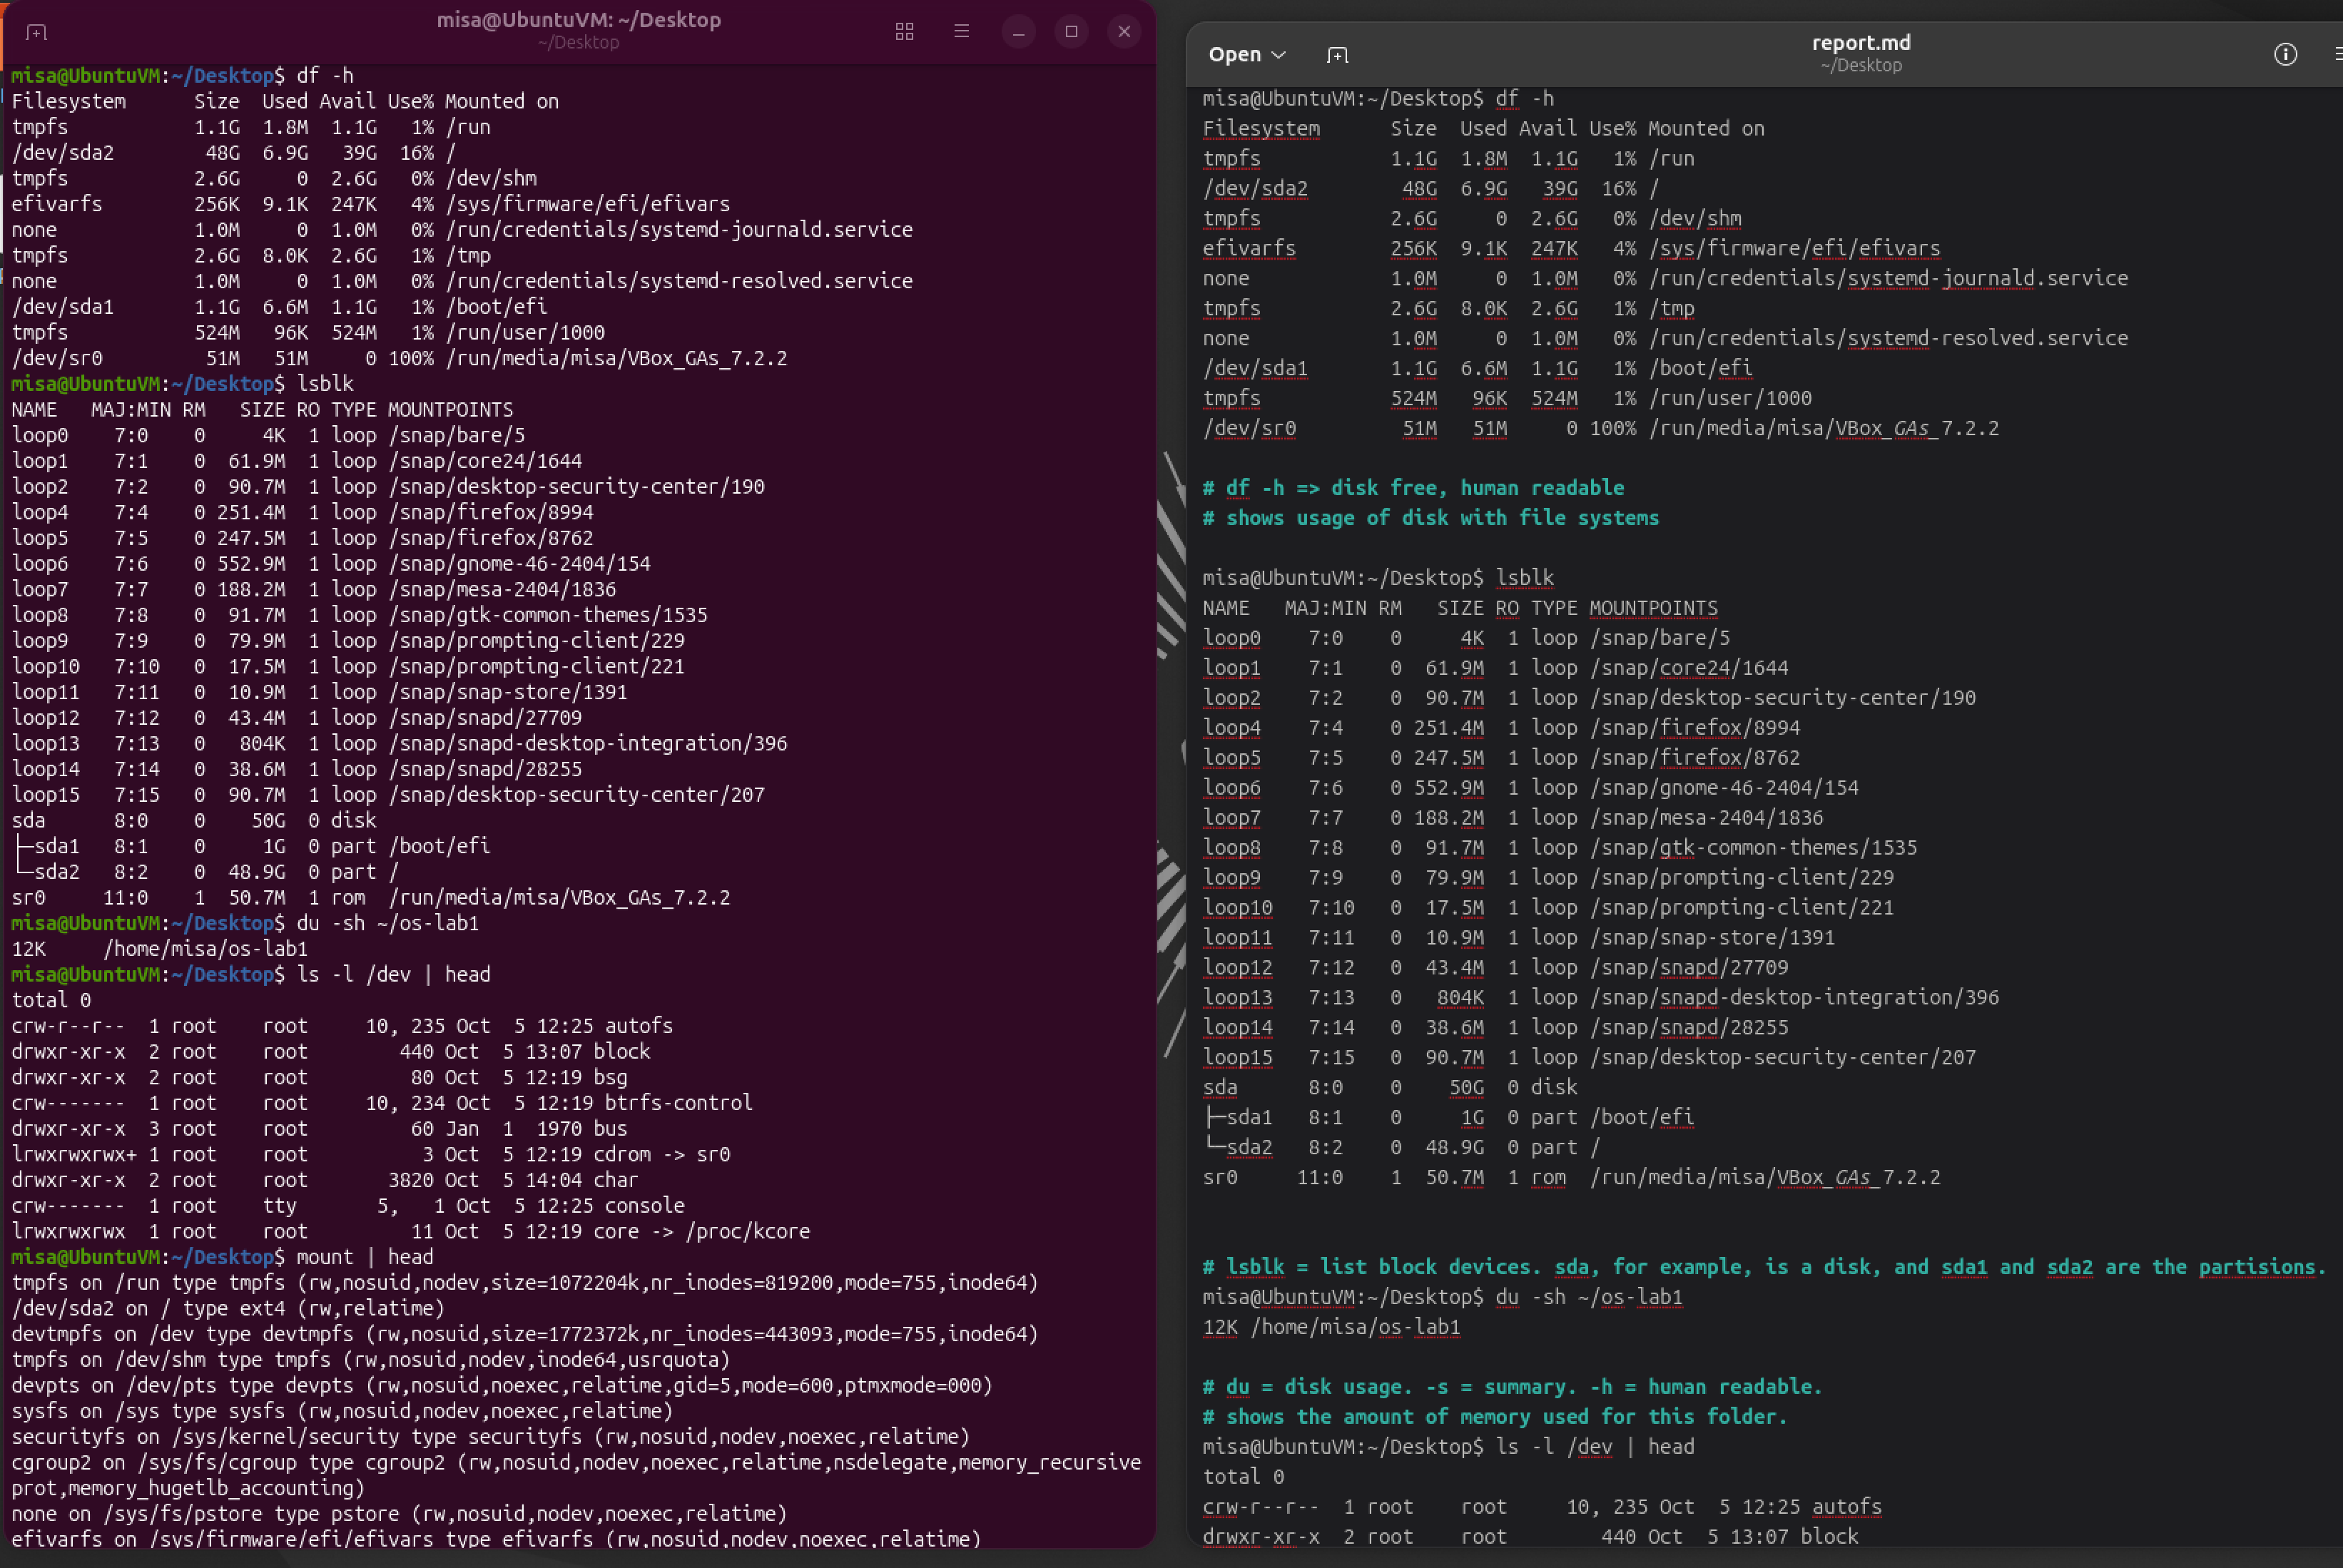
\includegraphics[width=0.82\textwidth]{./img/img_10.png}
    \caption{Devices and storage}
    \label{fig:label_10}
\end{figure}

\par We notice that the main disk \texttt{sda} has two partitions, with \texttt{/dev/sda2} containing the root filesystem \texttt{/} and \texttt{/dev/sda1} mounted at \texttt{/boot/efi}. The root filesystem has about 48 GiB of space, of which approximately 6.9 GiB is used. We can also notice that the \texttt{os-lab1} directory occupies only 12 KiB of disk space. The \texttt{/dev} directory provides file interfaces to devices; for example, \texttt{/dev/cdrom} represents the virtual CD/DVD drive, while \texttt{/dev/console} represents the system console and provides an interface for its input and output. The mounted filesystems show that different filesystems, such as \texttt{ext4}, \texttt{tmpfs}, \texttt{devtmpfs}, and \texttt{sysfs}, are attached to different points of the same directory tree. From this, we can notice the Unix concept that ``everything is a file'', meaning that Linux provides access to many system resources, including hardware devices, through a common file-like interface.

\clearpage

% =======================================================================
\chapter{CONCLUSIONS}
% =======================================================================


% =======================================================================
% =======================================================================

\par During this laboratory work, we observed how Linux manages four main system resources: files, processes, memory, and I/O devices. File management was explored using \texttt{ls -la}, which allowed us to inspect the file system, ownership, and permissions; process management was observed using \texttt{ps aux}, which showed the processes currently managed by the OS. Memory management was examined using \texttt{free -h}, which showed how physical RAM is distributed between used, free, and cached memory, while I/O devices and storage were explored using \texttt{df -h}, which showed the mounted filesystems and their disk usage. Overall, the laboratory work demonstrated how the operating system acts as a resource manager and provides common interfaces through which programs and users can interact with system resources.

\clearpage

% =======================================================================
% Bibliography
% =======================================================================

%\begin{thebibliography}{99}
\singlespace \normalsize

% \bibitem{ref:Chicago}
%   The Chicago Manual of Style.
%   "Notes and Bibliography: Sample Citations".
%   Accessed October 14, 2022.
%   \url{https://www.chicagomanualofstyle.org/tools_citationguide/citation-guide-2.html}.

% \bibitem{ref:Cats}
%   Google.
%   "Search results for cats".
%   Accessed August 15, 2023.
%   \url{https://www.google.com/search?q=cats}.

\bibitem{ref:OS-GfG}
  GeeksforGeeks.
  "What is an Operating System?".
  Last Updated July 25, 2025.
  Accessed October 16, 2025.
  \url{https://www.geeksforgeeks.org/operating-systems/what-is-an-operating-system/}.

\bibitem{ref:OS-concept}
Silberschatz, A., Galvin, P. B., \& Gagne, G. (2018).
\textit{Operating System Concepts} (10th ed.).
Wiley.
ISBN 978-1-119-32091-3.

\end{thebibliography}



\clearpage
\end{document}
